\appendix

% ------------------------------------------ CRM Data Facts
\chapter{Customer Journey}

Example of a \textit{customer journey} plot. Each dot represents an order made by the account, with a different color for each type of product. The number of weeks between an order and the previous one is written below each dot. The red dashed line on top of the plot indicates the volume of account reservoir. Monthly temperatures degrees and prices are also plotted.

\begin{figure}[htbp]
    \centering
    \hspace*{-1cm}
    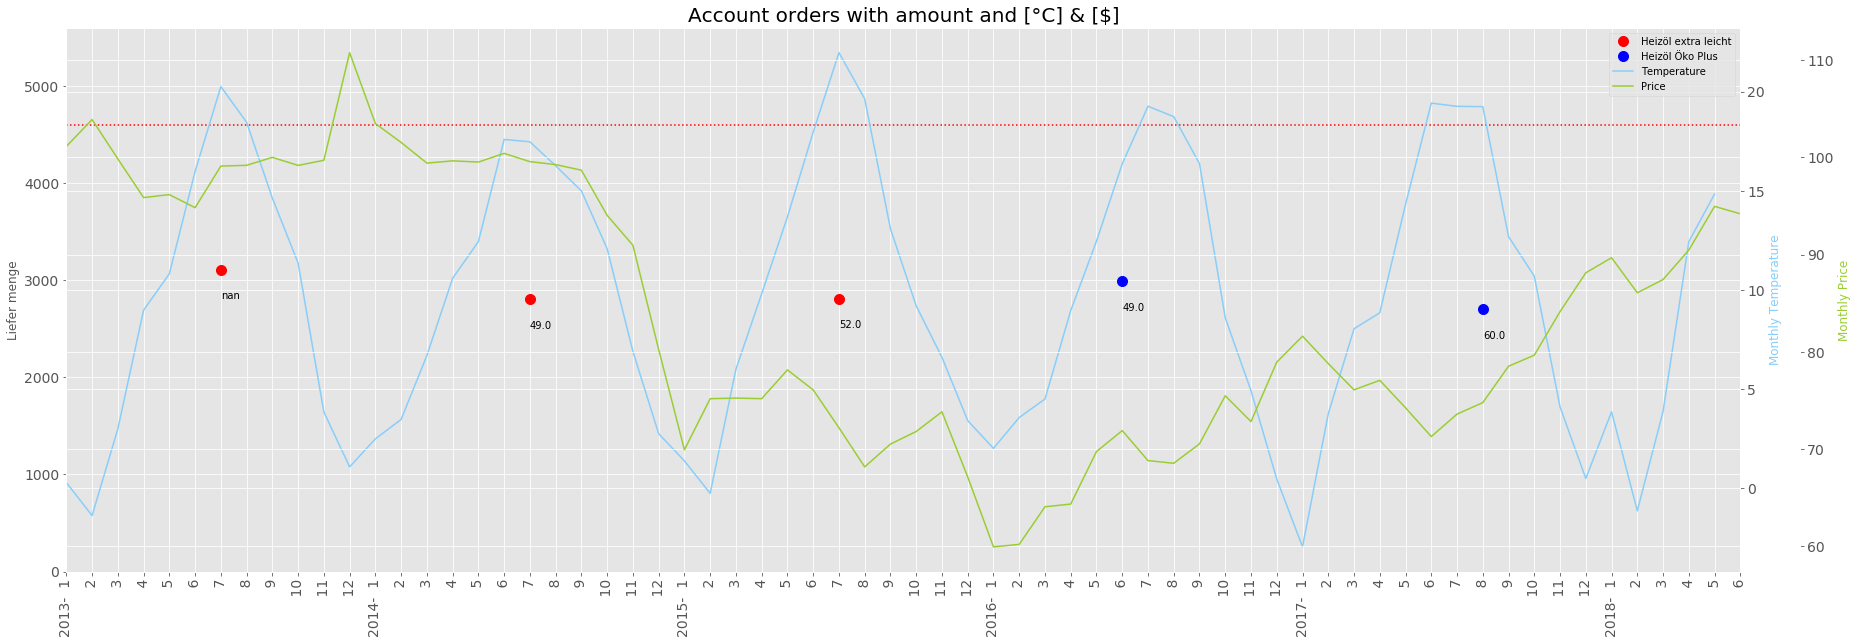
\includegraphics[width=17cm]{images/customer-journey.png}
    \caption{Example of a customer journey plot}
    \label{fig-annex:customer-journey}
\end{figure}


% ------------------------------------------ Features
\chapter{Features for machine learning}
\label{annex:features-for-ml}

{\footnotesize
    \begin{tabularx}{1\textwidth}{>{\bfseries}lL} 
        \\\toprule\endfirsthead
        \endhead
        \\ \multicolumn{2}{r}{\itshape continues on next page..}\\\midrule\endfoot
        \bottomrule\endlastfoot
         & \textbf{Account-related features} \\ \midrule
        1.  &   \textbf{account\_order\_id}        \tab   INTEGER     \tab   Number of orders made by the account before \\
        2.  &   \textbf{birth\_year}              \tab   INTEGER     \tab   Year of birth of the account. 0 if year not known \\
        3.  &   \textbf{member}                 \tab   BOOLEAN     \tab   Is account subscribe to the membership program \\
        4.  &   \textbf{email}                   \tab   BOOLEAN     \tab   Knowledge of the email for that account \\
        5.  &   \textbf{account\_type\_0..6}         \tab   ONE-HOT     \tab   Type of account \\
        6.  &   \textbf{name\_account}            \tab   BOOLEAN     \tab   Is account name null or not \\
        7.  &   \textbf{name\_account\_contact}    \tab   BOOLEAN     \tab   Are account and contact name the same \\
        8.  &   \textbf{name\_contact}            \tab   BOOLEAN     \tab   Is primary contact name null or not \\
        9.  &   \textbf{parent\_account}          \tab   BOOLEAN     \tab   Is an account with childs \\
        10.  &   \textbf{phone}                   \tab   BOOLEAN     \tab   Knowledge of account phone number \\
        11.  &   \textbf{language\_0..3}            \tab   ONE-HOT     \tab   Language of account \\
        12.  &   \textbf{tank\_type\_0..9}      \tab   ONE-HOT     \tab   Tank characteristic \\
        13.  &   \textbf{tank\_volumn}             \tab   FLOAT       \tab   Volumn capacity of customer tank \\
        
    \end{tabularx}

    %\pagebreak
    
    \begin{tabularx}{1\textwidth}{>{\bfseries}lL} 
        \small
        \\\toprule\endfirsthead
        \endhead
        \\ \multicolumn{2}{r}{\itshape continues on next page..}\\\midrule\endfoot
        \bottomrule\endlastfoot
         & \textbf{Current month features, with \textit{Weather} and \textit{Price}} \\ \midrule
        14.  &   \textbf{quantity\_coldays\_0}                           \tab   INTEGER \tab   Last order quantity delivered divided by 'nbr\_coldays\_below\_0' \\
        15.  &   \textbf{quantity\_coldays\_5}                         \tab   INTEGER \tab   Last order quantity delivered divided by 'nbr\_coldays\_below\_5' \\
        16.  &   \textbf{nbr\_coldays\_below\_0}*                     \tab   INTEGER \tab   Number of days with weather below 0 from last order until "today"   \\
        17.  &   \textbf{nbr\_coldays\_below\_5}*                     \tab   INTEGER \tab   Number of days with weather below 5 from last order until "today"   \\
        18.  &   \textbf{nbr\_months\_since\_last\_order}             \tab   FLOAT   \tab   Number of months (float) since previous account order   \\
        19.  &   \textbf{nbr\_weeks\_since\_last\_order}*              \tab   FLOAT   \tab   Number of weeks (float) since previous account order    \\
        20.  &   \textbf{nbr\_weeks\_left\_basedon\_prev}*             \tab   FLOAT   \tab   Number of weeks since last order    \\
        21.  &   \textbf{nbr\_months\_left\_basedon\_prev}*         \tab   FLOAT   \tab   Number of month since last order    \\
        22.  &   \textbf{nbr\_coldays0\_left\_basedon\_prev}*          \tab   INTEGER \tab   Number of days below 0 °C since last order minus number of days below 0 °C between last order and last last order   \\
        23.  &   \textbf{nbr\_coldays5\_left\_basedon\_prev}*         \tab   INTEGER \tab   Number of days below 5 °C since last order minus number of days below 5 °C between last order and last last order   \\
        24.  &   \textbf{nbr\_qtecoldays0\_left\_basedon\_prev}        \tab   FLOAT   \tab   Equation: df['prevqte\_coldays0']   -  df['qte\_coldays\_0']   \\
        25.  &   \textbf{nbr\_qtecoldays5\_left\_basedon\_prev}        \tab   FLOAT   \tab   Equation: df['prevqte\_coldays5']   -  df['qte\_coldays\_5']   \\
        26.  &   \textbf{price}                                          \tab   FLOAT   \tab   Current oil price   \\
        27.  &   \textbf{price\_past\_month\_0..9}                   \tab   FLOAT   \tab   Mean of the oil prices for XXX month ago    \\
        28.  &   \textbf{price\_past\_week\_0..3}                \tab   FLOAT   \tab   Mean of the oil prices for XXX week ago \\
        29.  &   \textbf{price\_prev\_diff\_01\_p}                \tab   FLOAT   \tab   Difference in percentage between current price and mean price of one month ago  \\
        30.  &   \textbf{price\_prev\_diff\_12\_p}                \tab   FLOAT   \tab   Difference in percentage between mean price of one month ago and mean price of 2 months ago \\
        31.  &   \textbf{price\_prev\_diff\_23\_p}                \tab   FLOAT   \tab   Difference in percentage between mean price of 2 months ago and mean price of 2 months ago  \\
        32.  &   \textbf{weather\_past\_month\_0..9}             \tab   FLOAT   \tab   Mean of the monthly weather of XXX month ago the last order \\
        33.  &   \textbf{weather\_past\_week\_0..3}              \tab   FLOAT   \tab   Mean of the weekly weather of XXX week ago the last order   \\
    \end{tabularx}
    
    %\pagebreak

    \begin{tabularx}{1\textwidth}{>{\bfseries}lL} 
        \small
        \\\toprule\endfirsthead
        \endhead
        \\ \multicolumn{2}{r}{\itshape continues on next page..}\\\midrule\endfoot
        \bottomrule\endlastfoot
         & \textbf{Features related to previous order} \\ \midrule
        34.  &    \textbf{account\_qte\_diff\_p\_mean}                             \tab   FLOAT   \tab   Difference in percentage between the previously delivered amount and the mean for this account \\
        35.  &    \textbf{account\_qte\_diff\_p\_median}                           \tab   FLOAT   \tab   Difference in percentage between the previously delivered amount and the median for this account \\
        36.  &    \textbf{account\_usage\_qtePerWeek\_diff\_p}                     \tab   FLOAT   \tab   Difference in percentage between the usage per week of the last order and the current usage per week \\
        37.  &    \textbf{elca\_datum\_month}                                        \tab   INTEGER \tab   Month number of account previous order (January -> 1, April -> 4, ...) \\
        38.  &    \textbf{elca\_datum\_week}*                                         \tab   INTEGER \tab   Week number of account previous order \\
        39.  &    \textbf{lieferqte2\_tankvolum}                                   \tab   FLOAT   \tab   Difference between (amount ordered+previous amount ordered) and tank volum for the last order in percents \\
        40.  &    \textbf{lieferqte\_tankvolum}                                    \tab   FLOAT   \tab   Difference between amount ordered and tank volum for the last order in percents \\
        41.  &    \textbf{quantity\_and\_days}                                          \tab   FLOAT   \tab   Theoretical number of days left based on amount of oil delivered in last order \\
        42.  &    \textbf{months\_until\_next\_theoritical\_order\_past\_order}*      \tab   FLOAT   \tab   Difference between the number of month between last and last last order and the number of months since last order \\
        43.  &    \textbf{months\_until\_next\_theoritical\_order\_account\_mean}    \tab   FLOAT   \tab   Mean of the number of months between two consecutive orders for each individual account \\
        44.  &    \textbf{months\_until\_next\_theoritical\_order\_account\_median}  \tab   FLOAT   \tab   Median of the number of months between two consecutive orders for each individual account \\
        45.  &    \textbf{order\_channel\_0..8}                                      \tab   ONE-HOT \tab   Channel for previous account's order \\
        46.  &    \textbf{prev\_delivery\_days}                                      \tab   INTEGER \tab   Number of days from last order and previous delivery (delivery of last last order) \\
        47.  &    \textbf{prev\_order\_days}                                         \tab   INTEGER \tab   Number of days from last order and last last order \\
        48.  &    \textbf{prev\_order\_months}                                       \tab   INTEGER \tab   Number of months from last order and last last order \\
        49.  &    \textbf{prev\_order\_weeks}*                                        \tab   INTEGER \tab   Number of weeks from last order and last last order \\
        50.  &    \textbf{previous\_qte}                                           \tab   FLOAT   \tab   Amount of oil of the last last order \\
        51.  &    \textbf{previous\_qte\_diff}                                     \tab   FLOAT   \tab   Difference in percentage between quantity delivered from last order and amount of the last last order \\
        52.  &    \textbf{prevqte\_coldays0}*                                       \tab   FLOAT   \tab   Amount delivered in last order divided by the number of days with weather below 0 \\
        53.  &    \textbf{prevqte\_coldays10}                                      \tab   FLOAT   \tab   Amount delivered in last order divided by the number of days with weather below 10 \\
        54.  &    \textbf{prevqte\_coldays5}*                                       \tab   FLOAT   \tab   Amount delivered in last order divided by the number of days with weather below 5 \\
        55.  &    \textbf{price\_ diff\_p}*                                           \tab   FLOAT   \tab   Difference in percentage between current order price and last order price \\
        56.  &    \textbf{price\_prev\_diff}                                         \tab   FLOAT   \tab   Difference between last order price and last last order price \\
        57.  &    \textbf{price\_prev\_diff\_p}*                                      \tab   FLOAT   \tab   Difference in percents between last order price and last last order price \\
        58.  &    \textbf{price\_prev\_diff\_w\_01\_p}*                               \tab   FLOAT   \tab   Difference in percentage between current price and mean price of one week ago \\
        59.  &    \textbf{price\_prev\_diff\_w\_12\_p}*                               \tab   FLOAT   \tab   Difference in percentage between mean price of 1 week ago and mean price of 2 weeks ago \\
        60.  &    \textbf{price\_prev\_diff\_w\_23\_p}                               \tab   FLOAT   \tab   Difference in percentage between mean price of 2 week ago and mean price of 3 weeks ago \\
        61.  &    \textbf{product\_0..6}                                             \tab   ONE-HOT \tab   Products ordered \\
        62.  &    \textbf{weather\_days\_below\_0}*                                   \tab   INTEGER \tab   Number of days below 0 °C between last order and last last order \\
        63.  &    \textbf{weather\_days\_below\_5}*                                   \tab   INTEGER \tab   Number of days below 5 °C between last order and last last order \\
        64.  &    \textbf{weather\_days\_below\_10}                                  \tab   INTEGER \tab   Number of days below 10 °C between last order and last last order \\
    \end{tabularx}
    
    
}



% --------------- NN experiments
\chapter{Neural Network experiments}
\label{annex:nn-experiments}

\textbf{Sketch of a simple neural network:}
\begin{figure}[h]
    \centering
    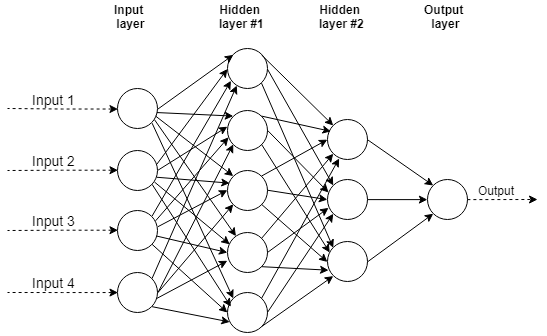
\includegraphics[width=10cm]{images/nn-sketch.png}
    \caption{Sketch a the Neural Network architecture composed of fully-connected layers.}
    \label{fig-annex:nn-sketch}
\end{figure}

\noindent\textbf{Models used:}\\
\texttt{Model 1}: One hidden layer composed of 90 neurons. \\
\texttt{Model 2}: One hidden layer composed of 200 neurons. \\
\texttt{Model 3}: Two hidden layers composed of 90 and 30 neurons respectively. \\
\texttt{Model 4}: Three hidden layers composed of 90, 60 and 30 neurons respectively. \\
\texttt{Model 5}: Three hidden layers composed of 200, 90 and 30 neurons respectively. \\

\pagebreak

\noindent\textbf{Set of features used:}\\
\texttt{Features 1}: Set of features composed of the entire XXX features created. \\
\texttt{Features 2}: Set of 41 features related to account, previous order and current month with price and weather data. \\
\texttt{Features 3}: Set of 10 features related to account, previous order and current month but without price and weather information. Based on results from Sklearn models.\\
\texttt{Features 4}: Set of 23 features similar to set 4 but with price and weather data. \\
\texttt{Features 5}: Set of 16 features similar to set 4 but with price data. \\
\texttt{Features 6}: Set of 19 features similar to set 4 but with weather data. \\


\noindent\textbf{Comments on table \ref{tab-annex:nn-experiments}}\\
\indent Models 6 and 5 are the two models with the better predictions. Those models are the most complete ones, with three hidden layers and it appears that the more neurons per hidden layer the best. In terms of running time, model 6 takes 2.5 more time to train per epoch.

After the model's architecture, the set of features is the most important parameter. Features set 3 and 4 are the one performing the best with models 5 and 6. Those sets are based on the best feature for the \textit{ExtraTree} model and for model 5 and 6, when weather and price related features are considered, the model performs slightly best. Based on the results obtain with feature set 5 and 6, it seems that weather-related features are more usefull to the predictions than price-related ones.

The feature set 4 contains the following features: 7, 14, 15, 18, 19, 20, 21, 24, 25, 34, 35, 39, 40, 41, 42, 43, 44, 48, 49, 51, 52, 53 and 54.


%\noindent\textbf{Results:}
\begin{table}[!h]
    \hspace{-6.6cm}\textbf{Results:}\\
    \centering
    \small
    \begin{tabular}{c|c|c|c|c|c}
        \textbf{Model} & \textbf{Features} & \textbf{Best epoch} & \textbf{Precision} & \textbf{Recall} & \textbf{F1-score} \\ \hline
        Model 6  &	Set 4      &	6	    &	0.791455    &	0.851300    &	0.820287    \\
        Model 6  &	Set 3      &	6	    &	0.815533    &	0.811962    &	0.813744    \\
        Model 6  &	Set 5      &	6	    &	0.781810    &	0.834485    &	0.807289    \\
        Model 5  &	Set 4      &	8	    &	0.806852    &	0.807025    &	0.806938    \\
        Model 5  &	Set 3      &	6	    &	0.795013    &	0.813357    &	0.804080    \\
        Model 6  &	Set 6      &	8	    &	0.826810    &	0.781778    &	0.803663    \\
        Model 4  &	Set 4      &	7	    &	0.803548    &	0.798725    &	0.801129    \\
        Model 4  &	Set 3      &	5	    &	0.802330    &	0.797961    &	0.800140    \\
        Model 4  &	Set 6      &	9	    &	0.807627    &	0.784523    &	0.795907    \\
        Model 5  &	Set 5      &	7	    &	0.803828    &	0.785380    &	0.794497    \\
        Model 5  &	Set 6      &	7	    &	0.821526    &	0.766461    &	0.793039    \\
        Model 4  &	Set 5      &	7	    &	0.783308    &	0.789053    &	0.786170    \\
        Model 5  &	Set 1      &	0	    &	0.814102    &	0.756303    &	0.784139    \\
        Model 6  &	Set 1      &	2	    &	0.791348    &	0.767504    &	0.779244    \\
        Model 2  &	Set 6      &	8	    &	0.781636    &	0.776302    &	0.778960    \\
        Model 2  &	Set 3      &	7	    &	0.771885    &	0.785075    &	0.778424    \\
        Model 1  &	Set 6      &	5	    &	0.779884    &	0.775070    &	0.777469    \\
        Model 3  &	Set 6      &	9	    &	0.772540    &	0.781452    &	0.776971    \\
        Model 2  &	Set 4      &	9	    &	0.756046    &	0.792444    &	0.773818    \\
        Model 3  &	Set 3      &	1	    &	0.778827    &	0.768450    &	0.773604    \\
        Model 3  &	Set 4      &	7	    &	0.767350    &	0.779901    &	0.773574    \\
        Model 2  &	Set 5      &	6	    &	0.772420    &	0.767589    &	0.769997    \\
        Model 1  &	Set 3      &	5	    &	0.763698    &	0.776149    &	0.769873    \\
        Model 1  &	Set 4      &	7	    &	0.748555    &	0.788513    &	0.768015    \\
        Model 4  &	Set 1      &	1	    &	0.772353    &	0.758589    &	0.765409    \\
        Model 3  &	Set 5      &	8	    &	0.739245    &	0.783388    &	0.760676    \\
        Model 1  &	Set 5      &	7	    &	0.761544    &	0.757843    &	0.759689    \\
        Model 4  &	Set 2      &	2	    &	0.689403    &	0.799537    &	0.740397    \\
        Model 6  &	Set 2      &	1	    &	0.660790    &	0.833442    &	0.737141    \\
        Model 5  &	Set 2      &	0	    &	0.666796    &	0.804559    &	0.729228    \\
        Model 3  &	Set 2      &	0	    &	0.678260    &	0.774853    &	0.723346    \\
        Model 3  &	Set 1      &	0	    &	0.733279    &	0.708292    &	0.720569    \\
        Model 1  &	Set 2      &	1	    &	0.669846    &	0.774422    &	0.718348    \\
        Model 2  &	Set 2      &	0	    &	0.656161    &	0.758358    &	0.703568    \\
        Model 2  &	Set 1      &	0	    &	0.717307    &	0.607880    &	0.658075    \\
        Model 1  &	Set 1      &	1	    &	0.672856    &	0.637357    &	0.654625    \\
    \end{tabular}
    \caption[Results for neural network architecture and features experiments]{Results for the model's architecture and features experiments. Scores retrieved with the testing dataset. Table sorted by decreasing Testing F1-score.}
    \label{tab-annex:nn-experiments}
\end{table}




% --------------- NN fine-tuning results
\chapter{Neural Network hyperparameters optimization}
\label{annex:nn-fine-tuning}

The hyperparameters tuning phase is decomposed into five parts, each part related to a parameter. Note that on the results below the best F1-score can be decreasing from one phase to another. This is a known issue with the Keras library: disregarding the seed for the random generator, there is still some level of randomness that cannot be avoided with the TensorFlow backend \cite{keras:seed-issue-blog,keras:seed-issue-github}. Nevertheless, models trained on the same script don't suffer from it.


\begin{enumerate}

    \item \textbf{Batch size} \\
        \vspace{-1cm}
        \begin{table}[htbp]
            \centering
            \begin{tabular}{c|c|c|c}
            \textbf{Batch size} & \textbf{Precision} & \textbf{Recall} & \textbf{F1-score} \\ \hline
                70      &	0.7952    &	0.8498    &	0.8216 \\
                150     &	0.7929    &	0.8467    &	0.8189 \\
                200     &	0.8077    &	0.8294    &	0.8184 \\
                100     &	0.8067    &	0.8268    &	0.8166 \\
                50      &	0.7938    &	0.8342    &	0.8135 \\
                10      &	0.8081    &	0.8191    &	0.8135 \\
                30      &	0.8014    &	0.8099    &	0.8057 \\
            \end{tabular}
        \end{table}        
    


    \item \textbf{Activation function}\\
        \vspace{-0.6cm}
        \begin{table}[htbp]
            \centering
            \begin{tabular}{l|c|c|c}
            \textbf{Activation} & \textbf{Precision} & \textbf{Recall} & \textbf{F1-score} \\ \hline
            elu         &	0.8140    &	0.8394    &	0.8265 \\
            selu        &	0.8076    &	0.8428    &	0.8248 \\
            softsign    &	0.8184    &	0.8138    &	0.8161 \\
            relu        &	0.8066    &	0.8103    &	0.8085 \\
            softplus    &	0.8239    &	0.7928    &	0.8081 \\
            tanh        &	0.8029    &	0.8056    &	0.8043 \\
            sigmoid     &	0.7888    &	0.8143    &	0.8013 \\
            softmax     &	0.8009    &	0.7635    &	0.7818 \\
            linear      &	0.5645    &	0.5851    &	0.7746 \\
            \end{tabular}
        \end{table}
    
    \item \textbf{Loss function}\\
        \vspace{-0.5cm}
        \begin{table}[htbp]
            \centering
            \begin{tabular}{l|c|c|c}
                \textbf{Loss function} & \textbf{Precision} & \textbf{Recall} & \textbf{F1-score} \\ \hline
                    logcosh &	0.7951    &	0.8661    &	0.8291 \\
                    msle    &	0.8044    &	0.8453    &	0.8243 \\
                    mae     &	0.8241    &	0.8239    &	0.8240 \\
                    mse     &	0.7442    &	0.8832    &	0.8078 \\
            \end{tabular}
        \end{table}
        
        
    \item \textbf{Optimizer}\\
        \vspace{-0.5cm}
        \begin{table}[htbp]
            \centering
            \begin{tabular}{l|c|c|c}
                \textbf{Optimizer} & \textbf{Precision} & \textbf{Recall} & \textbf{F1-score} \\ \hline
                    adamax  &	0.8002    &	0.8319    &	0.8156 \\
                    adam    &	0.8266    &	0.8006    &	0.8133 \\
                    sgd     &	0.7959    &	0.8097    &	0.8028 \\
                    adagrad &	0.7744    &	0.8284    &	0.8005 \\
            \end{tabular}
        \end{table}


    \item \textbf{Bias usage}\\
        \vspace{-0.5cm}
        \begin{table}[htbp]
            \centering
            \begin{tabular}{l|c|c|c}
                \textbf{Bias} & \textbf{Precision} & \textbf{Recall} & \textbf{F1-score} \\ \hline
                True    &	0.8044    &	0.8427    &	0.8231 \\
                False   &	0.8118    &	0.8210    &	0.8164 \\
            \end{tabular}
        \end{table}
        
        
    \end{enumerate}


% --------------- LSTM results
\chapter{LSTM experiments}
\label{annex:lstm-experiments}


\textbf{Sketch of a neural network with an LSTM layer:}
\begin{figure}[h]
    \centering
    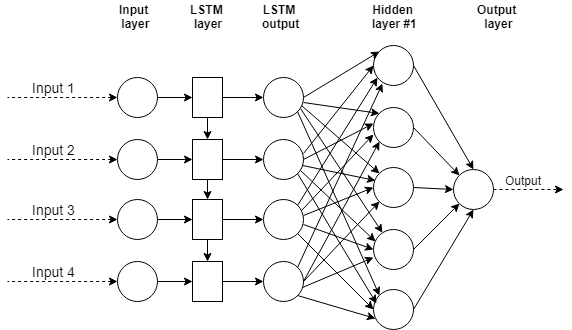
\includegraphics[width=10cm]{images/nn-sketch-lstm.png}
    \caption[Sketch of a Neural Network with LSTM layer]{Sketch of a the Neural Network architecture composed of an LSTM layer and one fully-connected layer afterwards.}
    \label{fig-annex:nn-sketch-lstm}
\end{figure}

\noindent\textbf{Models used}\\
\texttt{Model 1}: LSTM layer with an output of size 90 without  fully connected layers. \\
\texttt{Model 2}: LSTM layer with an output of size 200 without fully connected layers. \\
\texttt{Model 3}: LSTM layer with an output of size 90 followed by a fully connected layer with 60 neurons. \\
\texttt{Model 4}: LSTM layer with an output of size 90 followed by three fully connected layers with 200, 100 and 50 neurons \\
\texttt{Model 5}: Two stack LSTM layers with size of 100 and 50 without fully connected layers. \\


\textbf{Results:}
\begin{table}[htbp]
    \centering
    \small
    \begin{tabular}{c|c|c|c|c|c}
        \textbf{Model} & \textbf{Features} & \textbf{Best epoch} & \textbf{Precision} & \textbf{Recall} & \textbf{F1-score} \\ \hline
        Model 4    &	Set 6	    &   4      &      0.853547     &	0.756196    &	0.801928  \\
        Model 4    &	Set 5	    &   3      &      0.851867     &	0.757161    &	0.801727  \\
        Model 4    &	Set 3	    &   8      &      0.831043     &	0.770204    &	0.799468  \\
        Model 4    &	Set 2	    &   9      &      0.858899     &	0.746690    &	0.798874  \\
        Model 4    &	Set 4	    &   9      &      0.860676     &	0.745085    &	0.798720  \\
        Model 5    &	Set 6	    &   5      &      0.839094     &	0.743312    &	0.788304  \\
        Model 4    &	Set 1	    &   9      &      0.812634     &	0.765249    &	0.788230  \\
        Model 3    &	Set 2	    &   5      &      0.852265     &	0.732955    &	0.788120  \\
        Model 5    &	Set 3	    &   8      &      0.836295     &	0.739536    &	0.784945  \\
        Model 5    &	Set 2	    &   8      &      0.834816     &	0.735545    &	0.782043  \\
        Model 3    &	Set 6	    &   5      &      0.818325     &	0.746955    &	0.781013  \\
        Model 2    &	Set 4	    &   8      &      0.820919     &	0.744311    &	0.780740  \\
        Model 2    &	Set 3	    &   8      &      0.792452     &	0.766322    &	0.779168  \\
        Model 2    &	Set 2	    &   6      &      0.755777     &	0.801203    &	0.777827  \\
        Model 3    &	Set 5	    &   9      &      0.845743     &	0.719995    &	0.777819  \\
        Model 1    &	Set 6	    &   9      &      0.796770     &	0.758796    &	0.777320  \\
        Model 3    &	Set 3	    &   6      &      0.825161     &	0.733698    &	0.776746  \\
        Model 5    &	Set 5	    &   7      &      0.836228     &	0.724553    &	0.776395  \\
        Model 2    &	Set 6	    &   9      &      0.818859     &	0.736902    &	0.775722  \\
        Model 1    &	Set 2	    &   7      &      0.786494     &	0.764248    &	0.775211  \\
        Model 5    &	Set 1	    &   8      &      0.803029     &	0.748767    &	0.774949  \\
        Model 5    &	Set 4	    &   4      &      0.843988     &	0.715625    &	0.774524  \\
        Model 3    &	Set 4	    &   3      &      0.830222     &	0.721050    &	0.771795  \\
        Model 2    &	Set 1	    &   5      &      0.786466     &	0.749751    &	0.767670  \\
        Model 1    &	Set 5	    &   8      &      0.821374     &	0.719641    &	0.767149  \\
        Model 2    &	Set 5	    &   8      &      0.793832     &	0.741482    &	0.766765  \\
        Model 3    &	Set 1	    &   7      &      0.817767     &	0.721585    &	0.766671  \\
        Model 1    &	Set 4	    &   6      &      0.806085     &	0.726495    &	0.764223  \\
        Model 1    &	Set 3	    &   7      &      0.795377     &	0.734691    &	0.763830  \\
        Model 1    &	Set 1	    &   9      &      0.767634     &	0.742091    &	0.754646  \\
    \end{tabular}
    \caption[LSTM models results]{Results obtain by LSTM-base neural networks. Scores obtains with the testing dataset. Ranked by decreasing F1-score.}
    \label{tab-annex:nn-experiments-lstm}
\end{table}


\noindent\textbf{Comments:}\\
It's clear that Model 4 performs the best. This is the most complete model, with three fully connected hidden layers following the LSTM one. Compared to previous neural network models without an LSTM, the \texttt{Precision} metric achieves a better score. When looking at the detailed score, LSTM models perform much better with the $t_0\_p_0$ metric: it indicates that the predictions are "precise" and would perform the best if the model's one-month tolerance is dropped.